%%
%% This is file `sample-sigconf.tex',
%% generated with the docstrip utility.
%%
%% The original source files were:
%%
%% samples.dtx  (with options: `sigconf')
%% 
%% IMPORTANT NOTICE:
%% 
%% For the copyright see the source file.
%% 
%% Any modified versions of this file must be renamed
%% with new filenames distinct from sample-sigconf.tex.
%% 
%% For distribution of the original source see the terms
%% for copying and modification in the file samples.dtx.
%% 
%% This generated file may be distributed as long as the
%% original source files, as listed above, are part of the
%% same distribution. (The sources need not necessarily be
%% in the same archive or directory.)
%%
%% Commands for TeXCount
%TC:macro \cite [option:text,text]
%TC:macro \citep [option:text,text]
%TC:macro \citet [option:text,text]
%TC:envir table 0 1
%TC:envir table* 0 1
%TC:envir tabular [ignore] word
%TC:envir displaymath 0 word
%TC:envir math 0 word
%TC:envir comment 0 0
%%
%%
%% The first command in your LaTeX source must be the \documentclass command.
\PassOptionsToPackage{table,xcdraw}{xcolor}
\documentclass[sigconf, nonacm]{acmart}
%% NOTE that a single column version may be required for 
%% submission and peer review. This can be done by changing
%% the \doucmentclass[...]{acmart} in this template to 
%% \documentclass[manuscript,screen]{acmart}
%% 
%% To ensure 100% compatibility, please check the white list of
%% approved LaTeX packages to be used with the Master Article Template at
%% https://www.acm.org/publications/taps/whitelist-of-latex-packages 
%% before creating your document. The white list page provides 
%% information on how to submit additional LaTeX packages for 
%% review and adoption.
%% Fonts used in the template cannot be substituted; margin 
%% adjustments are not allowed.
%%
%%
%% \BibTeX command to typeset BibTeX logo in the docs
\AtBeginDocument{%
  \providecommand\BibTeX{{%
    \normalfont B\kern-0.5em{\scshape i\kern-0.25em b}\kern-0.8em\TeX}}}

%% Rights management information.  This information is sent to you
%% when you complete the rights form.  These commands have SAMPLE
%% values in them; it is your responsibility as an author to replace
%% the commands and values with those provided to you when you
%% complete the rights form.
\setcopyright{none}
\copyrightyear{2022}
\acmYear{2022}
\acmDOI{XXXXXXX.XXXXXXX} 

%% These commands are for a PROCEEDINGS abstract or paper.
\acmConference[Conference acronym 'XX]{Make sure to enter the correct
  conference title from your rights confirmation emai}{June 03--05,
  2018}{Woodstock, NY}
%
%  Uncomment \acmBooktitle if th title of the proceedings is different
%  from ``Proceedings of ...''!
%
%\acmBooktitle{Woodstock '18: ACM Symposium on Neural Gaze Detection,
%  June 03--05, 2018, Woodstock, NY} 
\acmPrice{15.00}
\acmISBN{978-1-4503-XXXX-X/18/06}


%%
%% Submission ID.
%% Use this when submitting an article to a sponsored event. You'll
%% receive a unique submission ID from the organizers
%% of the event, and this ID should be used as the parameter to this command.
%%\acmSubmissionID{123-A56-BU3}

%%
%% For managing citations, it is recommended to use bibliography
%% files in BibTeX format.
%%
%% You can then either use BibTeX with the ACM-Reference-Format style,
%% or BibLaTeX with the acmnumeric or acmauthoryear sytles, that include
%% support for advanced citation of software artefact from the
%% biblatex-software package, also separately available on CTAN.
%%
%% Look at the sample-*-biblatex.tex files for templates showcasing
%% the biblatex styles.
%%

%%
%% The majority of ACM publications use numbered citations and
%% references.  The command \citestyle{authoryear} switches to the
%% "author year" style.
%%
%% If you are preparing content for an event
%% sponsored by ACM SIGGRAPH, you must use the "author year" style of
%% citations and references.
%% Uncommenting
%% the next command will enable that style.
%%\citestyle{acmauthoryear}

%%
%% end of the preamble, start of the body of the document source.

%% Removing ACM Reference Format
\settopmatter{printacmref=false}

\begin{document}

%%
%% The "title" command has an optional parameter,
%% allowing the author to define a "short title" to be used in page headers.
\title{Kernel methods for protein classification}

%%
%% The "author" command and its associated commands are used to define
%% the authors and their affiliations.
%% Of note is the shared affiliation of the first two authors, and the
%% "authornote" and "authornotemark" commands
%% used to denote shared contribution to the research.
\author{Jérémie Dentan}
\email{jeremie.dentan@polytechnique.org}
\affiliation{%
  \institution{École Polytechnique}
}

%%
%% By default, the full list of authors will be used in the page
%% headers. Often, this list is too long, and will overlap
%% other information printed in the page headers. This command allows
%% the author to define a more concise list
%% of authors' names for this purpose.
\renewcommand{\shortauthors}{Dentan}

%%
%% The abstract is a short summary of the work to be presented in the
%% article.
\begin{abstract}

Protein classification is a crucial task bio-informatics and computational biology, especially in drug discovery. The structure of proteins, as 3D folded sequence of amino acids, determines their specific chemical functionalities. The aim of this project is to apply kernel methods on the graph structure of a number of proteins to classify them into 2 classes.

Our approach has been to implement five different type of kernel on the protein graphs, and four different type of kernel classifiers, and to try all the combinations between those kernels and those classifiers, using several hyperparameters for each of them.

For the kernels, we implemented: (1) a kernel based on the histograms of the edge labels, (2) a kernel based on the histograms of the vertex labels, (3) a kernel based on the concatenation of those two histograms, (4) the Pyramid Match kernel \cite{grauman_pyramid_2007} with 8 different hyperparameters, and (5) the Shortest Path kernel \cite{borgwardt_shortest-path_2005}.

For the classifiers, we implemented: (1) an unweighted K-Nearest-Neighbor (KNN), (2) a weighted KNN with a linear weight depending on the rank of the neighbor, (3) a weighted KNN with hyperbolic weight depending on the distance of the neighbor, and (4) a Kernel Support Vector Machine (K-SVM). For the three KNN, we used 58 different hyperparameters, varying the number of neighbors from 3 to 60, and for the K-SVM, we used 11 different hyperparameter for the tuple of the weight on the constraint and the number of training point.

In the end, we tested 12 different kernels configuration and 185 different classifiers configuration, for a total of 2220 combination. This thorough study allowed us to reach satisfactory performances considering the difficulty of the challenge: we obtained an AUC score of 81\% and a ranking of 14 out of 22.

\end{abstract}

%%
%% Keywords. The author(s) should pick words that accurately describe
%% the work being presented. Separate the keywords with commas.

%\received{01 January 2023}
%\received[revised]{12 March 2009}
%\received[accepted]{5 June 2009}

%%
%% This command processes the author and affiliation and title
%% information and builds the first part of the formatted document.
\maketitle

\section{Introduction}

The code of all our implementation is available in \href{https://github.com/DentanJeremie/kernel-proteins}{\underline{this repository}}.

\subsection{The challenge}

The challenge consists in a binary classification task on proteins 3D configuration. There are 6000 training proteins, and 2000 proteins for which we have to do the prediction. The configuration of the proteins is given in the form of a graph representing the interractions between the amino acids. The labels of the nodes represent features on the chemical bonds between these elements, while the labels between the edges represent features on the amino acids themselves. 

The challenge evaluation metric is the AUC score associated with the logits predicted on the test set. Moreover, the challenge imposed to used kernel methods only to solve the problem.

A first difficulty related to these datasets is that the organizers of the challenge did not disclose the biological meaning represented by these different features or by the two classes to predict. This was done to make the task more complicated, however this omission prevents us from performing the most important part of any machine learning problem, namely the fine understanding of the data at stake via exchanges with domain experts.

\subsection{Data exploration}

First, we briefly explored the data at hand:

\begin{itemize}
    \item The data are highly imbalanced, with more than 90\% of the proteins belonging to the same class (cf. figure \ref{fig:data_histo}, left). Given the algorithms we deployed, which are not very amenable to this problem of imbalance, the only thing we did for this was to create a subset whose classes are balanced, and which we used as a training set for K-SVM.
    \item The distribution of the edges labels is similar between the train and test set (cf. figure \ref{fig:data_histo}, right). Thus, we do not have to deal with a distribution shift.
\end{itemize}


\begin{figure}[t]
    \centering
    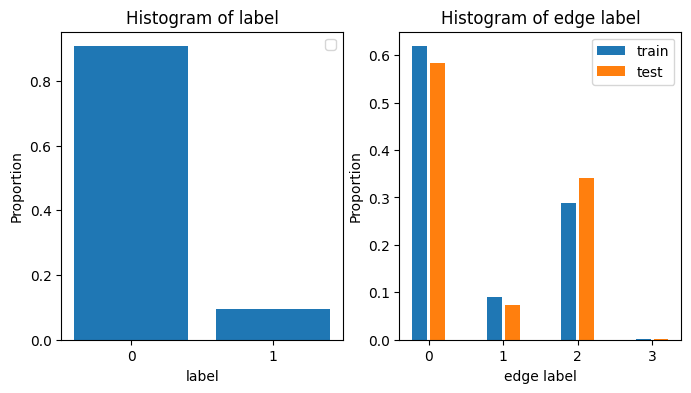
\includegraphics[width=\columnwidth]{figures/histograms.png}
    \caption{Left: histogram of the labels in the train set. Right: Histogram of the edge labels.}
    \label{fig:data_histo}
\end{figure}

\subsection{Related work}

Machine Learning (ML) techniques for protein classification have received a lot of interest in the past years, mainly due to its huge industrial applications. Indeed, conducting experiments to study the properties of an unknown protein is an extremely time consuming and costly task. Thus, ML models can interestingly filter proteins in order to conduct biological experiments on promising proteins only \cite{naik_active_2016}.

Some surveys have been conducted on protein classification, such as \cite{gupta_protein_2019}, but they do not specifically focus on kernel methods. However, we can mention that kernel methods were already used on proteins, both on their sequences of amino-acid or on their spacial configuration \cite{vert_classification_2006, ben-hur_kernel_2005}.

Finally, there exist some interesting and comprehensive survey on graph kernels, such as \cite{nikolentzos_graph_2021}. We used this survey to choose which kernel to implement.

\section{Our algorithms}

In this section, we present the kernels we computed on the proteins, as well as the classifier we used with those kernels.

\subsection{Our kernels}

\paragraph{Histogram-based kernels}

The first kernels we implemented are really simple, based on the histograms of node labels and edge labels. For example, for the node labels, there are $50$ possible label for each node, so each graph $G$ is mapped to a point $\phi(G) \in \mathbb{R}^{50}$ corresponding to the histogram of each label in this graph. For this kernel, $\mathbb{R}^{50}$ is the RKHS of the kernel, and its natural dot product defines the kernel evaluation between two graphs. We did the same for edge histogram, the concatenation of those two histograms.

$$K(G_1, G_2) = <\phi(G_1), \phi(G_2)>$$

\paragraph{Pyramid Match kernel} 

Then, due to its very good performances announced in \cite{nikolentzos_graph_2021}, we decided to implement the Pyramid-Match kernel \cite{grauman_pyramid_2007}. This kernel first embeds each node of each graph in a $d$-dimension space using the eigenvalues of the adjacency matrix. Then, the kernel evaluation between two graph is computed using the histogram that count how many of the nodes in this $d$-dimension space fall into the same cell. The size of these cells involves an additional parameter, called the level and noted $l$.

We tested 8 combination of parameter, making $d$ varying between $3$ and $6$, and $l$ varying between $3$ and $4$.

\paragraph{Shortest Path kernel}

Similarly, due to its good performances announced in \cite{nikolentzos_graph_2021}, we implemented the Shortest Path kernel \cite{borgwardt_shortest-path_2005}. This kernel first computes the shortest path between all points in all graphs, and then the kernel evaluation between two graphs is computed using the histogram of shortest path length classified according to the labels of the nodes at the ends of the shortest paths.

For this kernel, we can vary how the histograms are compared, but we decided not to introduce any hyperparameter here.

\subsection{Our classifiers}

\paragraph{Kernel-KNN}

First, we used three type of KNN to predict the logit of the classification on the test set:
\begin{itemize}
    \item A simple unweighted KNN, for wich the final logit is the weighted average of the class of the neighbors
    \item A weighted KNN with linear weights, each neighbor having weight $1-k/N$ where $k$ is the rank of the neighbor and $N$ the number of neighbor used.
    \item A weighted KNN with hyperbolic weights, with each neighbor having weight $1/d_k$ where $d_k$ is the distance between neighbor $k$ and the querry point.
\end{itemize}

For each of those classifier, we made the number of neighbor vary from 3 to 60, resulting in a total of 174 classifier tested.

\paragraph{Kernel-SVM}

Then, we used a regular kernel SVM classifier, solving the following minimization problem:

$$
\min_{f, b, \xi_i} \frac{1}{2}||f||^2 + c \sum_i\xi_i
$$
$$
\text{s. t. } y_i(f(x_i) + b) \ge 1 - \xi_i \ ; \ \xi_i \ge 0 
$$

Where $x_i$ are the embedded values in the RKHS (not computed), and $y_i$ their labels. To reduce computation time, we restrained the number of points in the train set, and used a balanced subset between the two classes. Thus, there are two hyperparameters for this method: the value of $c$, and the number of training points. We used 11 different configuration for those hyperparameters.

\subsection{Choosing the best configuration}

As said above, we tested all combination of our 12 kernels and 185 classifiers, leading to 2220 possibilities. Thus, we needed a way to choose which one was the best and submit it for the challenge. To do so, we randomly extracted 1000 graphs out of the 6000, and used it as a validation set that was never used during training.

\subsection{Hardware and computation time}

For our experiments, we used a Intel Xeon W-1290P 3.70GHz, using a single process. For both the Pyramid Match and Shortest Path kernel, the computation of the Gram matrix for our 8000 points took about 20min per kernel. In each case, the preprocessing steps (computing shortest paths, or eigenvalue decomposition) were really fast, and the slowest was the pairwise comparison of the histograms. On the contrary, the computation of the simple histogram kernels was really fast, about few seconds.

Then, for the classifiers, all classifier were really fast (the bottleneck was the disk writing of the output), except the K-SVM, which took about 20sec per fitting.

Finally, all our experiments took about 2h45 of computation.

\section{Conclusion}

The approach described above enable us to reach a final AUC score of 81\% and a ranking of 14 out of 22, which is quite satisfying with respect to the difficulty of the challenge. This best AUC score was achieve using the Pyramid Match kernel with $d = 4$ and $l = 4$, with a hyperbolic-weighted KNN using 26 neighbors.


%%
%% The next two lines define the bibliography style to be used, and
%% the bibliography file.
\bibliographystyle{ACM-Reference-Format}
\bibliography{references}


\end{document}
\endinput
%%
%% End of file `sample-sigconf.tex'.
